\section{Methodology}
\subsection{Procedure}
The procedure used in this research is as follows:
\begin{enumerate}
	\item Use a mutation testing tool (PIT) to produce faulty program and run it against master test suite. Get mutant status for every test case.
	\item Generate a large number of test suites by randomly selecting tests cases from master test suite, until the test suite reaches its pre-defined size.
	\item For each test suite:
	\begin{itemize}
		\item Measure coverage criteria (CodeCover) for different test suites.
		\item Determine effectiveness of different test suites using mutation information and coverage criteria.
	\end{itemize}
	\item Analyse correlation between different coverage criteria and effectiveness.
\end{enumerate}

\subsection{Subjects under test}
The original paper used five following subject programs: 
\begin{enumerate}
	\item Apache POI~\cite{apachepoi}: a Java API for Microsoft Documents
	\item Closure~\cite{closure}: a tool for making JavaScript download and run faster.
	\item HSQLDB~\cite{hsqldb}: a Java SQL relational database.
	\item JfreeChart~\cite{jfreechart}: a Java chart library for users to display professional quality charts.
	\item Joda Time~\cite{jodatime}: A replacement for Java time and date class
\end{enumerate}

These five subjects are selected on purpose using the following criteria:
\begin{enumerate}
	\item The program needs to be large enough to have more than 100,000 SLOC;
	\item It needs to be an actively developed Java program;
	\item It contains at least 1000 test cases;
	\item The project needs to use Ant as its build system;
	\item The project uses JUnit as a test harness.
\end{enumerate}

However no versions or git hashes of subject programs were given in the original paper or in its artefact page. As the original paper was published in 2014, various number of test subjects versions between 2012 to 2014 were examined with different PIT versions, but there was no result that was close enough to what was reported in the original paper. Figure~\ref{fig:jodamutant} and figure~\ref{fig:jodakilled} are examples of different versions of Joda Time running against PIT version 1.0.0. We contacted authors of the original paper, and acquired their project repository.


\begin{figure}
	\centering
	\begin{minipage}{0.4\textwidth}
		\centering
		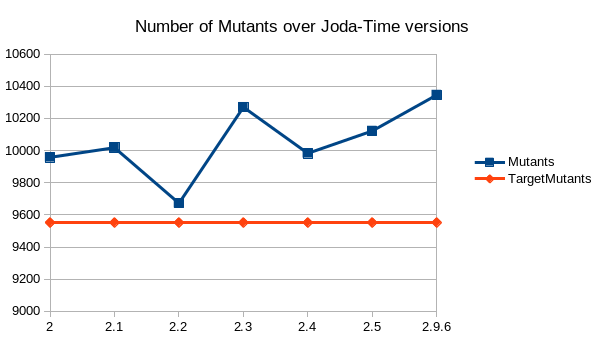
\includegraphics[width=\textwidth]{Figure/joda_mutant.png}
		\caption{Joda Time total mutants}
		\label{fig:jodamutant}
	\end{minipage} %
	\begin{minipage}{0.4\textwidth}
		\centering
		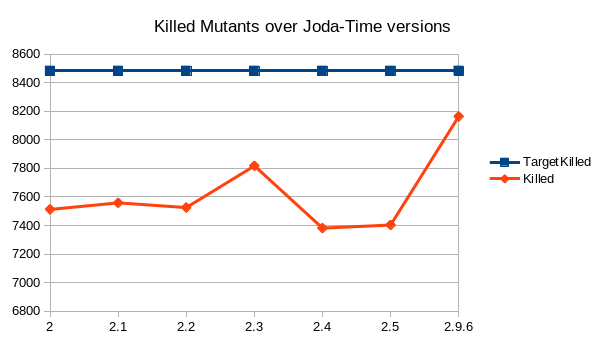
\includegraphics[width=\textwidth]{Figure/joda_kill.png}
		\caption{Joda Time killed mutants}
		\label{fig:jodakilled}
	\end{minipage}
\end{figure}

There are some environment settings need to be adjusted locally. Mutation testing tool PIT used for this project requires green test suite, which means all tests must pass. During my replication, some projects provided by the author could not compile or did not pass all tests. The first Java compiler used in the replication was Java 8, but non of the projects passed all tests. HSQLDB, JfreeChart, Joda Time worked with no errors using Java 7. According to ant build system, recommanded Java compiler for Closure was Java 6, but non of the compiler version complied it successfully. For Apache POI, Java 6 and 7 compilation was successful but resulted failing tests.

There was no command to exclude failing tests in author's repository, and the report log suggests the Apache POI and Closure were working correctly. I downloaded source code from GitHub according to author's repository. Table~\ref{tab:sut} is a summary of projects and compiler version. Java 7 was selected as final replication compiler.


\begin{table}
	\caption{Java Compiler Setting}
	\label{tab:sut}
	\begin{minipage}{\columnwidth}
		\begin{center}
			\begin{tabular}{|l|l|c|c|c|c|c|c|}
				\hline
				&&\multicolumn{2}{|c|}{Java 6}&\multicolumn{2}{|c|}{Java 7}&\multicolumn{2}{|c|}{Java 8}\\
				\hline
				Project & Version & Compile & Test & Compile & Test & Compile & Test \\
				\hline
				Apache POI & 3.9(author) & Success & Fail & Success & Fail & Success & Fail \\
				& 3.9(GitHub) & Success & Success& Success& Success & Success& Fail \\
				\hline
				Closure& 20130227(author) & Fail & Fail & Fail & Fail & Fail & Fail \\
				&20130227(GitHub) & Success & Success & Success & Success & Success & Fail \\
				\hline
				HSQLDB & 2.2.8 & Success & Success & Success & Success & Success & Fail \\
				\hline
				JfreeChart & 1.0.8 & Success & Success & Success & Success & Success & Fail \\
				\hline
				Joda Time & 2.0 & Success & Success & Success & Success & Success & Fail \\
				\hline
			\end{tabular}
		\end{center}
		\bigskip
	\end{minipage}
\end{table}

The final environment settings used in this replication study are:
\begin{itemize}
	\item Operating System: Ubuntu 14.04.5 LTS;
	\item Java Compiler: 1.7.0\_u131;
	\item ant build system: 1.9.3;
	\item JUnit: 3.8 for compiling projects, 4.10 for running PIT;
	
Other systems should work, as long as using Java compiler 7, ant version greater than 1.8; and having JUnit 3 and JUnit 4  at the same time.
\end{itemize}


\subsection{Mutation Testing}
Mutation testing of the program was conducted using an automated mutilation testing tool PIT, which is one of the most widely used open source Java mutation testing system. Version of PIT used for the original paper was 0.30-SNAPSHOT. PIT run tests against automatically generated mutants. Firstly it performs statement coverage for the tests, then use coverage information to pick test cases targeting a particular mutant.

For a mutant, PIT report one of the following result status:
\begin{itemize}
	\item Killed: mutant has been killed by the test suite.
	\item Live: mutant has survived.
	\item No coverage: no test case executed the line of code where the mutant was created.
	\item Time out: the mutants causes an infinite loop, for example mutate loop counter in a for loop.
	\item Non viable: the mutant is invalid and can not be loaded by the Java Virtual Machine (JVM).
	\item Memory error: the mutation requires more memory to be used by system.
	\item Run error: there is something wrong when running the mutant.	
\end{itemize}

Under normal circumstances, there should be no non viable mutants or errors.

Although author did not mention in the paper, she has made some modification to PIT. For the original PIT, if a mutant is killed by a test case, the test case is logged, then PIT moves to next mutant. So in the final report, only the first test case killed the mutant was reported. For the modified  PIT, a mutant run against all possible test cases target it, PIT moves to next mutant when all covered test cases are executed, and result for every test case and its corresponding mutant is logged in a log file. The modification is valid for 4 out of 5 subjects, but generated different results for HSQLDB compare to original PIT report. This will be discussed in more detail in section~\ref{subsec:resultPIT}

\subsection{Test suite generation}

\subsection{Coverage Measurement}
Coverage criteria are measured using an open source Java coverage analysis tool CodeCover. Statement, decision and modified condition types are used in the project.

Statement coverage is measured for the following statement type:
\begin{itemize}
	\item assignments and method calls
	\item variable and member declaration with an assignment
	\item break
	\item continue
	\item return
	\item throw
	\item empty statements
\end{itemize}

All condition statements such as if and for are not considered for statement coverage.

Decision branches are measured for the branches:
	\begin{itemize}
		\item if-else statements, which have one branch for if and another for else
		\item switch-case statements have a branch for each case and one for default
		\item try-catch statements have a bran for every catch, one branch for exceptions not in catch cases and one branch for successful execution.
	\end{itemize}

MCC coverage consider the boolean expressions in:
	\begin{itemize}
		\item if
		\item for
		\item while and do...while
	\end{itemize}
Boolean expressions not in decision or looping statements are ignored, such as assignments and method parameters.
\subsection{Measuring Effectiveness}